% !TEX TS-program = pdfLaTeX+shellescape
% !TEX encoding = UTF-8 Unicode

\documentclass{standalone}
\usepackage{pgfplots}
\pgfplotsset{compat=1.17}
\usepackage{amssymb}
\usetikzlibrary {arrows.meta}

\definecolor{tab_blue}{HTML}{1F77B4}
\definecolor{tab_orange}{HTML}{FF7F0E}

\begin{document}
    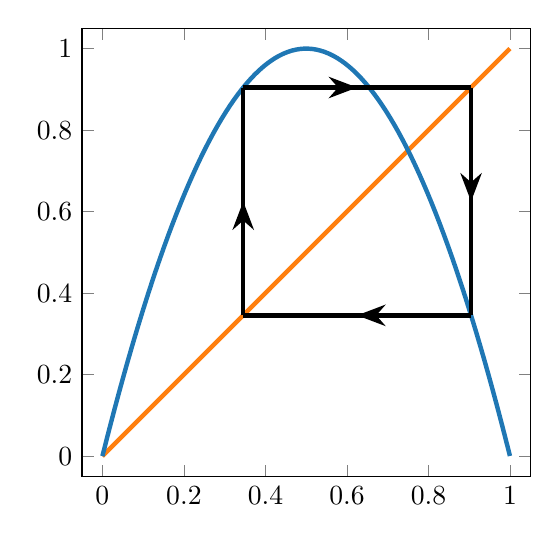
\begin{tikzpicture}[baseline]
        \begin{axis}[
            scale=1, % scale
            xmin=-0.05,xmax=1.05,ymin=-0.05,ymax=1.05, % range of plot
            % legend style={at={(axis cs: 1,0)}, anchor=south east}, % position of legends
            unit vector ratio = {1, 1}, % aspect ratio
            axis lines = box, % middle or box
            %axis x line = bottom, % top, middle, bottom, none: axis x line* = ... removes arrow heads
            %axis y line = left, % left, center, right, none: axis y line* = ... removes arrow heads
            % xlabel = {$x$}, % axis labels 
            % xtick = {-10},
            % y axis line style = {draw=none},
            % ytick = {-10},
        ]
            \addplot[color=tab_orange, samples=22, domain=0:1, ultra thick] {x};
            \addplot[color=tab_blue, samples=100, domain=0:1, ultra thick] {4*x*(1-x)};
            \draw[color=black, ultra thick] ({(5+sqrt(5))/8}, {(5+sqrt(5))/8}) -- ({(5+sqrt(5))/8}, {(5-sqrt(5))/8});
            \draw[color=black, ultra thick] ({(5+sqrt(5))/8}, {(5-sqrt(5))/8}) -- ({(5-sqrt(5))/8}, {(5-sqrt(5))/8});
            \draw[color=black, ultra thick] ({(5-sqrt(5))/8}, {(5-sqrt(5))/8}) -- ({(5-sqrt(5))/8}, {(5+sqrt(5))/8});
            \draw[color=black, ultra thick] ({(5-sqrt(5))/8}, {(5+sqrt(5))/8}) -- ({(5+sqrt(5))/8}, {(5+sqrt(5))/8});
            \draw[-Stealth, color=black, ultra thick] ({(5+sqrt(5))/8}, {(5+sqrt(5))/8}) -- ({(5+sqrt(5))/8}, {5/8});
            \draw[-Stealth, color=black, ultra thick] ({(5+sqrt(5))/8}, {(5-sqrt(5))/8}) -- ({5/8}, {(5-sqrt(5))/8});
            \draw[-Stealth, color=black, ultra thick] ({(5-sqrt(5))/8}, {(5-sqrt(5))/8}) -- ({(5-sqrt(5))/8}, {5/8});
            \draw[-Stealth, color=black, ultra thick] ({(5-sqrt(5))/8}, {(5+sqrt(5))/8}) -- ({5/8}, {(5+sqrt(5))/8});
            
        \end{axis}
    \end{tikzpicture}
    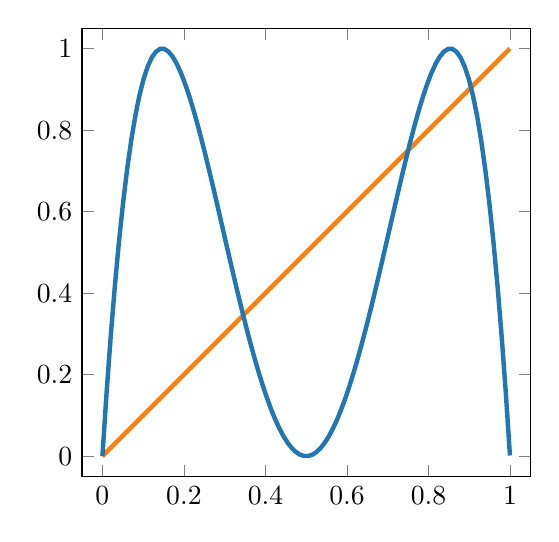
\begin{tikzpicture}[baseline]
        \begin{axis}[
            scale=1, % scale
            xmin=-0.05,xmax=1.05,ymin=-0.05,ymax=1.05, % range of plot
            % legend style={at={(axis cs: 1,0)}, anchor=south east}, % position of legends
            unit vector ratio = {1, 1}, % aspect ratio
            axis lines = box, % middle or box
            %axis x line = bottom, % top, middle, bottom, none: axis x line* = ... removes arrow heads
            %axis y line = left, % left, center, right, none: axis y line* = ... removes arrow heads
            % xlabel = {$x$}, % axis labels 
            % xtick = {-10},
            % y axis line style = {draw=none},
            % ytick = {-10},
        ]
            \addplot[color=tab_orange, samples=22, domain=0:1, ultra thick] {x};
            \addplot[color=tab_blue, samples=100, domain=0:1, ultra thick] {4*4*x*(1-x)*(1-4*x*(1-x))};
        \end{axis}
    \end{tikzpicture}
    
\end{document}